%%%%%%%%%%%%%%%%%%%%%%%%%%%%%%%%%%%%%%%%%%%%%%%%%%%%%%%%%%%%%%%%%%%%%%%
%%%%%%%%%%%%%%%%%%%%%%%%%%%%%%%%%%%%%%%%%%%%%%%%%%%%%%%%%%%%%%%%%%%%%%%
%%%%%                                                                 %
%%%%%     <file_name>.tex                                             %
%%%%%                                                                 %
%%%%% Author:      <author>                                           %
%%%%% Created:     <date>                                             %
%%%%% Description: <description>                                      %
%%%%%                                                                 %
%%%%%%%%%%%%%%%%%%%%%%%%%%%%%%%%%%%%%%%%%%%%%%%%%%%%%%%%%%%%%%%%%%%%%%%
%%%%%%%%%%%%%%%%%%%%%%%%%%%%%%%%%%%%%%%%%%%%%%%%%%%%%%%%%%%%%%%%%%%%%%%


\noindent\textbf{Processor Model: }The platform considered consists of two cores, as shown in Figure~\ref{fig:system_model}. Both cores have same microarchitecture, but different power consumption due to different timing closures. The \textit{Heavy Core} (HC) is designed under worst-case design margins and is guaranteed to work at the maximum frequency $F_{\mathrm{HC}}$. The \textit{Light Core} (LC) is designed with reduced design margins and is not guaranteed to operate at $F_\mathrm{HC}$. However, it is guaranteed to operate at a lower frequency $F_{\mathrm{LC}}\leq F_{\mathrm{HC}}$. 
%Thirdly, the processor also consists of peripherals with non-negligible power consumption.  
%The system model that we study in this semester thesis is actually the model proposed in \cite{Gomez1, Gomez2}. It is inspired by heterogeneous dual-core MCUs, such as the \emph{LPCXpresso54102}, which we used as the emulation platform. 
%\begin{figure}[!htbp]
%  \centering
%  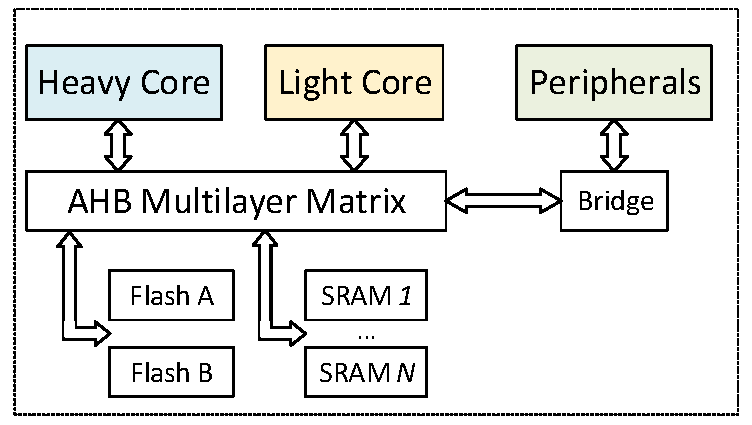
\includegraphics[scale=1]{./figures/system_model}
%  \caption{Hardware Architecture of proposed dual-core platform.}
%  \label{fig:system_model}
%\end{figure}
%As shown in Figure~\ref{fig:system_model}, the platform consists of two cores featuring the same ISA. The first core has been designed under the worst-case design margins, whereas the second one has been implemented to work under more relaxed operating conditions. In this semester thesis, we call the first core \emph{Heavy Core (HC)} and the second one \emph{Light Core (LC)}. The \emph{HC} is guaranteed to work at its maximum frequency (\emph{$F_{max}$}) with a probability of \emph{100\%}. On the other hand, the \emph{LC} might not always be able to reach the \emph{$F_{max}$}, but it is guaranteed to work at a frequency \emph{$F_{LC} \leq F_{max}$}, independently of the operating conditions. Moreover, the \emph{LC} is much more energy-efficient, because of its relaxed design margins, which means that when the two cores operate at the same frequency, the LC consumes less energy. The presence of the \emph{HC} provides some minimum performance guarantees and by offloading tasks to the \emph{LC}, we can improve substantially the energy consumption of the platform.\par


\begin{figure}[!tbp]
	\centering
	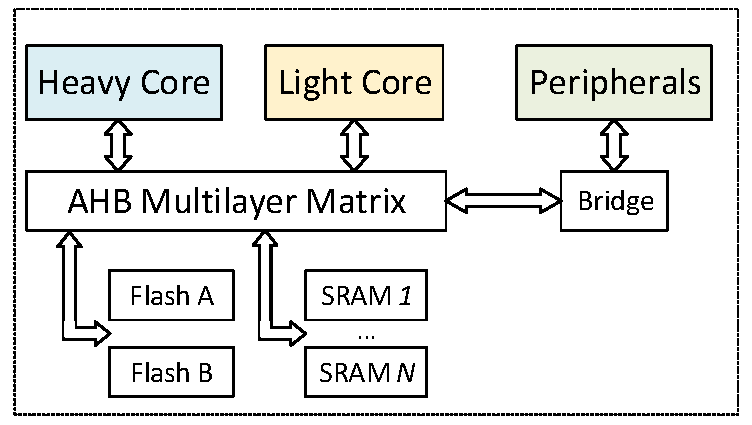
\includegraphics[width=0.7\linewidth]{./figures/system_model}
	\caption{Architecture of proposed dual-core platform.}
	\label{fig:system_model}
\end{figure}

\noindent\textbf{Power Model: }The system power consumption can be divided into three main components: the power consumption of the HC ($P_\mathrm{HC}$), the power consumption of the LC ($P_\mathrm{LC}$) and the power consumption of the system peripherals ($P_\mathrm{Sys}$). Due to reduced design margins, LC is more energy efficient compared to the HC. This implies that even when HC and LC operate at the same frequency, $P_\mathrm{LC}\leq P_\mathrm{HC}$. Each component has two different states: \emph{active} and \emph{sleep}. The sleep power of all components is non-negligible; however, it is constant. This constant factor is ignored in all power/energy computations in the remaining paper. Therefore, $P_\mathrm{X}=P_\mathrm{X,Active} - P_\mathrm{X,Sleep}\;, X\in\{\mathrm{HC}, \mathrm{LC}, \mathrm{SYS}\}$. The peripherals can be put into sleep only when both cores are in sleep state. 
%It is assumed that $P_\mathrm{Sys}$ is comparable to $P_\mathrm{HC}$. 
Formally, we focus on Heavy-Light platforms that operate under the following three conditions:\\
\textbf{Condition 1}: $F_\mathrm{HC}\geq F_\mathrm{LC}\geq \displaystyle\frac{ F_\mathrm{HC}}{2}$\\\\
\textbf{Condition 2}: $\displaystyle\frac{F_\mathrm{LC}}{P_\mathrm{LC}}\geq \displaystyle\frac{F_\mathrm{HC}}{P_\mathrm{HC}}$\\\\ 
\textbf{Condition 3}: $P_{\mathrm{HC}}\leq P_{\mathrm{LC}}+ P_{\mathrm{Sys}}$\\\\
%where: $P_\mathrm{X}=P_\mathrm{X,Active} - P_\mathrm{X,Sleep}\;, X\in\{\mathrm{HC}, \mathrm{LC}, \mathrm{SYS}\}$\\\\
Condition 1 emphasizes that LC might have performance penalty, due to its relaxed design margins. Condition 2 implies that LC is more energy efficient compared to HC, given that sleep powers are much smaller compared to active powers. Finally, condition 3 states that the power consumption of the peripherals is comparable to the power consumption of the HC. Previous works have shown that low power MCU platforms satisfy these conditions \cite{Gomez1, Fuks}.

\noindent\textbf{Task Model: }Applications consist of a set of \textit{n} periodic and independent tasks. It is assumed that all tasks have the same period $D$. Furthermore, it is assumed that all tasks are atomic units of execution; thus, preemptions and migrations are not allowed. This is a fairly restrictive assumption; however, it is realistic for deeply low power MCU platforms. $C_i$ is used to denote the computation cycles of task $i$.


%Studies have shown that in power-constrained MCU platforms, $E_{Sys}$ is comparable to $E_{HC}$. Therefore, our proposed solutions try to improve the energy consumption by minimizing the active time of the peripherals ($A_{SYS}$), as shown in Figure~\ref{fig:comparison}.
%\begin{figure}[!htbp]
%  \centering
%  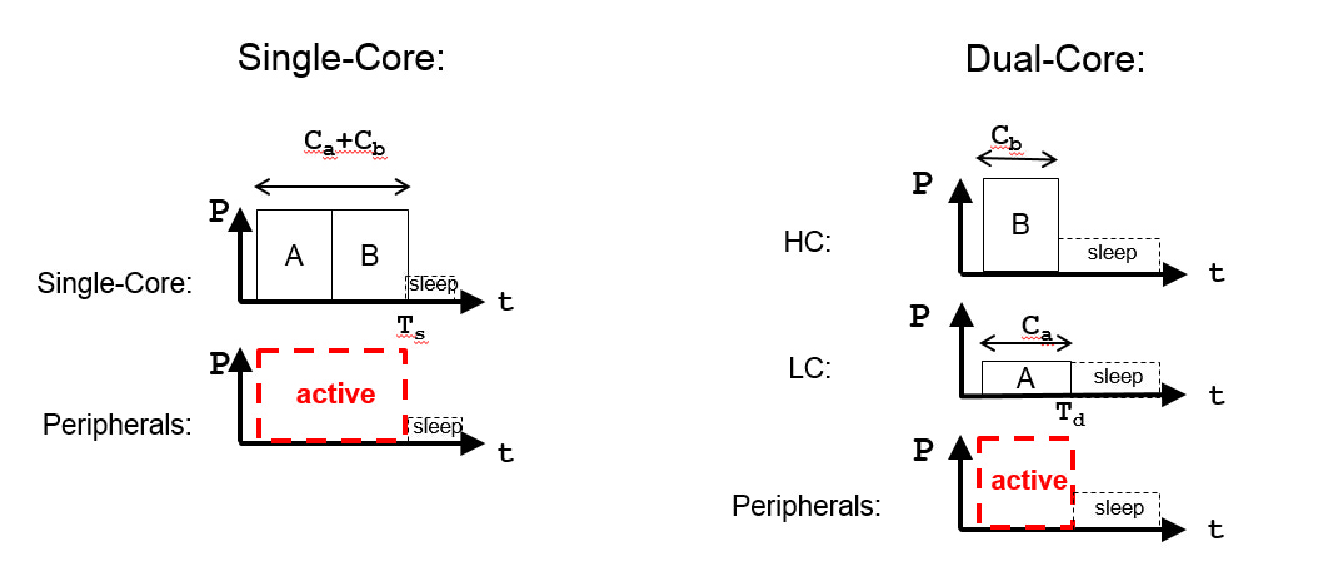
\includegraphics[width=\linewidth]{./figures/Comparison}
%  \caption{Comparison of a single-core and the proposed dual-core platform.}
%  \label{fig:comparison}
%\end{figure}

%\par
%The main advantages of the proposed architecture compared to the alternatives are the homogenous ISA and the energy efficiency offered by the \emph{LC}. This is in contrast to the modern dual-core MCU platforms which exploit the architectural heterogeneity in order to decrease the energy consumption. Due to architectural heterogeneity, the coprocessor cannot run the same applications as the main processor, rendering the platform inflexible. Dynamic allocation policies cannot be applied and any parallelization scheme has to be applied statically at design time. However, this is not a problem for the proposed architecture, as the two cores have the same ISA and thus they can allow more complex task allocation algorithms and parallelization schemes.\par

